\documentclass[tikz,border=10pt]{standalone}
\usepackage{tikz}
\usetikzlibrary{shapes.geometric, arrows.meta, positioning, calc, fit, backgrounds}

\begin{document}
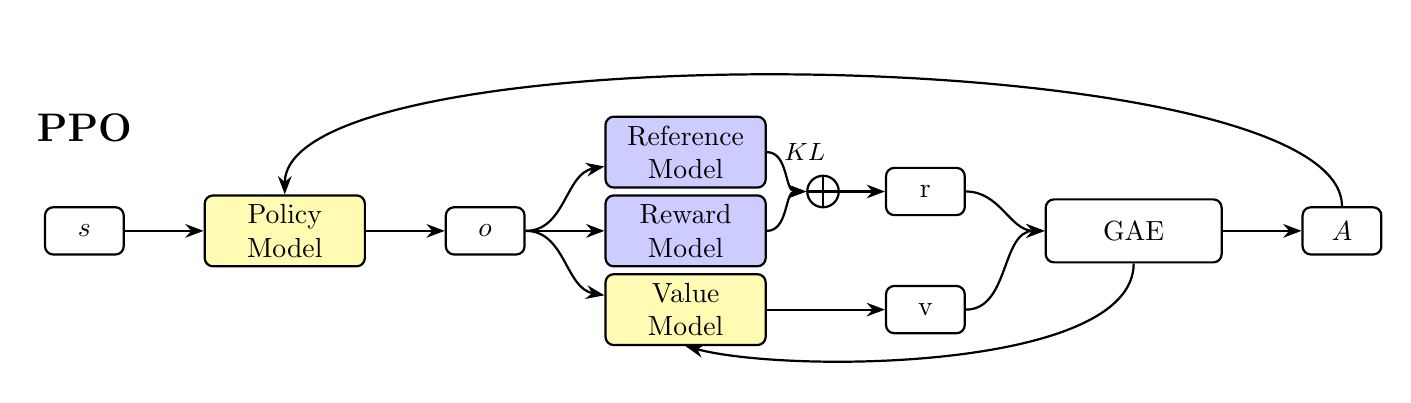
\begin{tikzpicture}[
    % Define styles
    box/.style={rectangle, draw=black, thick, minimum width=2cm, minimum height=0.8cm, rounded corners=3pt, text width=1.8cm, align=center},
    model/.style={box, fill=blue!20},
    policy/.style={box, fill=yellow!30},
    compute/.style={box, minimum width=2.2cm, text width=2cm},
    small/.style={box, minimum width=1cm, minimum height=0.6cm, text width=, align=center},
    plus/.style={circle, draw=black, thick, minimum size=0.4cm, fill=white, path picture={\draw[black, thick] (path picture bounding box.north) -- (path picture bounding box.south) (path picture bounding box.west) -- (path picture bounding box.east);}},
    arrow/.style={->, >=Stealth, thick},
    group_box/.style={rectangle, draw=gray!60, thick, fill=gray!10, rounded corners=5pt, inner sep=8pt},
    ]

    % Main nodes
    \node[small] (s) at (0, 0) {$s$};
    \node[font=\Large\bfseries] at ($(s.north) + (0,1.0)$) {PPO};
    \node[policy, right=1cm of s] (policy) {Policy\\Model};

    % Action samples from Policy Model
    \node[small, right=1cm of policy] (o) {$o$};


    \node[model, right=1cm of o, yshift=1.0cm] (ref) {Reference\\Model};
    \node[model, right=1cm of o] (reward) {Reward\\Model};
    % Value Model
    \node[policy, right=1cm of o, yshift=-1.0cm] (value) {Value\\Model};

    % Plus node (circular with cross)
    \node[plus, right=0.5cm of reward, yshift=0.5cm] (plus) {};
    
    % KL label
    \node[right=0.1cm of ref, font=\small] {$KL$};

    % Value outputs
    \node[small, right=1.5cm of value] (v) {v};
    \node[small, right=1.5cm of reward, yshift=0.5cm] (r) {r};

    % PPO Computation
    \node[compute, right=1cm of v, yshift=1.0cm] (GAE) {GAE};

    \node[small, right=1cm of GAE] (A) {$A$};

    % Arrows
    \draw[arrow] (s) -- (policy);
    \draw[arrow] (policy) -- (o);

    % Arrows from action group to models
    \draw[arrow] (o) to[out=0, in=170] (value);
    \draw[arrow] (o) to[out=0, in=180] (reward);
    \draw[arrow] (o) to[out=0, in=190] (ref);

    % Arrows from models to outputs
    \draw[arrow] (value) to[out=0, in=180] (v);
    \draw[arrow] (reward) to[out=0, in=180] (plus);
    \draw[arrow] (ref) to[out=0, in=180] (plus);
    \draw[arrow] (plus) -- (r);

    \draw[arrow] (r) to[out=0, in=180] (GAE);
    \draw[arrow] (v) to[out=0, in=180] (GAE);

    \draw[arrow] (GAE) to[out=0, in=180] (A);

    \draw[arrow] (A.north) to[out=90, in=90, looseness=0.4] (policy.north);
    \draw[arrow] (GAE.south) to[out=270, in=-15, looseness=0.6] (value.south);



\end{tikzpicture}
\end{document}